%\chapter{How to Use Sombrero}
\section{Admin Mode}
\subsection{What is Admin Mode?}

  If you are logged in as a user with superuser privileges, you are considered to be in admin mode. In admin mode, you are able to do everything a normal user can, but you are shown some additional input elements for managing the room/widget layout and general server setup. Thus, for the purpose of this chapter, it is assumed you are familiar with user mode controls. If there are currently no users with admin privileges, which is most commonly the case after setup if no users have been created yet, all users can be created with admin privileges or take admin privileges through the edit user form. Admin can also give admin privileges to other users through the userlist.

  In admin mode, you can create rooms and widgets through the admin sidebar in room view. Similarly, individual widgets can be modified using the widget configuration buttons while in room view. To configure users and reset passwords, use the user list. To configure the KNX router used to access the KNX network, use the router discovery. To easily add knx widgets, use the device finder. Finally, to set KNX address aliases to match your group address setup, use the KNX group page.

  \clearpage
\subsection{Widget Editing}

  As the widget editing dialog can appear in different places and sometimes different forms, here is a list of widget attributes:
  \begin{itemize}
    \item \textbf{Name:} The name of the widget, which is useful for identifying it among widgets of the same class. It cannot be blank, and while it is possible to give different widgets the same name, it is discouraged to do so.
    \item \textbf{Class:} The class of the widget, or in other words, what this widget represents. Possible values are either different types of KNX widgets (e.g. Lamps or Temperature) and room links. Depending on the class of the widget, the other attributes may change.
    \item \textbf{Attributes of KNX widgets:}
    \begin{itemize}
      \item \textbf{Group Address:} KNX group address of the represented device. If you don't have your devices' group address information at hand, it is perhaps easier to use the device finder.
      \item \textbf{KNX Groups:} Additional KNX group addresses of the device. This is needed to correctly display the device's state.
    \end{itemize}
    \item \textbf{Attributes of Room Links:}
    \begin{itemize}
      \item \textbf{Room Reference:} The room this link leads to when clicked.
      \item \textbf{Image:} The image that is displayed on this room link. It should help to quickly identify the linked room.
    \end{itemize}
  \end{itemize}

\subsection{Admin Sidebar}

  The admin sidebar has two major areas: room modification and the widget clipboard, which can be shown using the upper and lower buttons on the right side of the screen respectively. The room modification area contains forms for adding child rooms to the current room, adding widgets to the current room, directly modifying the current rooms attribute, and deleting the current room.

  You can quickly add widgets too rooms using the widget adding area. Just fill in all the fields, hit "Add Widget", and the widget will appear in the current room. For information on what to enter into the specific fields, see widget editing\ref{NEEDED}.

  The room adding area is used to add rooms to your current layout. Rooms can be used to group widgets and other rooms to mimic their physical layout for easier identification. The room attribute modification area has the same fields, but the changes are applied to the current room instead of a new one. Room rooms can be added in the index page, accessible through the Sombrero logo on the upper left.
  \begin{itemize}
    \item \textbf{Name:} The name of the room. It is the only information the user has of a room when navigating, so choose a meaningful name. It cannot be blank, and while it is possible to give different rooms the same name, it is discouraged to do so.
    \item \textbf{Image:} The background image that is shown when the user visits the room. A good idea is to use a photograph of the room or its floor plan in order to allow users to arrange widgets according to their physical position.
  \end{itemize}

  The widget clipboard is where widgets not currently associated with a room appear. It's handling is similar to the favourites bar. Widgets can be stored here and put back into rooms using the Widget configuration buttons. It should be empty most of the time, as users without admin privileges cannot access the contained widgets.

\subsection{Widget Configuration Buttons}

  While in admin mode, every widget has a configuration bar. It consists of 4 small icons with various functionalities.
  \begin{itemize}
    \item 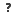
\includegraphics{admin-help.png} displays a help page
    \item 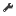
\includegraphics{admin-edit.png} opens the widget editing dialog
    \item 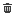
\includegraphics{admin-delete.png} deletes the widget. Deleted widgets cannot be restored, so be careful.
    \item 
\includegraphics{admin-plus.png} 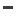
\includegraphics{admin-minus.png} removes the widget from the current room and adds it to the clipboard, or vice-versa.
  \end{itemize}

\subsection{User List}

  The user list is the admin's tool to edit other user's accounts. In the column on the left, the user's email addresses are listed. By clicking one of them, you are shown the user editing form known from user mode, but for another user than yourself. By using the password boxes and the "Set Password" button, you can reset user passwords in case someone forgot it. The "Delete User" button deletes the corresponding user. You can even delete other administrators and once deleted, users cannot be recovered, so be careful.

\subsection{Router Discovery}

  This is the page that allows you to view and change the IP address of the KNX router used to access your KNX network. This step is crucial for Sombrero as it is impossible to access any KNX device without it. In most home networks, it will be enough to just hit the "Start Discovery" button and click the first router IP address that pops up. If more than one IP addresses appear, you have more than one KNX router in your network and need to decide which one to use. You can also set the router IP directly via the textbox and the "Set Router IP" button.

\subsection{Device Finder}

  The device finder provides an easy interface for adding KNX widgets when the group addresses are not known (or hard to find). Just press the "Start Device Finder" button and send some KNX commands using other hardware, e.g. switch your light on with the appropriate switch. Addresses which receive 3 or more commands are shown in a list, along with the amount of commands received. Click one of the KNX addresses, and you are presented with a KNX widget adding form. Once the widget is saved, it appears in the clipboard and can be added to the room of your choice.

\subsection{Group Address Aliases}

  KNX group address aliases are needed to correctly identify the device or devices a message is heading to if a device has more than one address. KNX group address alias configuration consists of to two steps.

  First, you have to define the KNX alias addresses. To do this, head to the "KNX Groups". Enter the names and addresses of KNX groups present in your physical setup. Names are just for identification and should be chosen accordingly.

  Second, you have to set the groups your widgets are in. Once you define one or more KNX groups, they appear as checkboxes in the widget editing form. Just check the groups your widget belongs to and save.
